\section*{Frequency Domain Enhancement}

\subsection*{Fourier Transform}

\textbf{Idea:} Any function that periodically repeats itself
can be expressed as a sum of sines and cosines of different
frequencies each multiplied by a different coefficient

\begin{figure}[H]
  \includegraphics[width=\linewidth]{images/fourier.png}
  \caption{A wave (top) and its Fourier components (bottom)}
\end{figure}

\subsubsection*{Discrete Fourier Transform (DFT)}

\textit{Discrete Fourier Transform} of $f(x, y)$ for $x = 0 \ldots
M-1$ and $y = 0 \ldots N-1$ is defined as:
\begin{equation*}
  F(u, v) = \sum_{x=0}^{M-1} \sum_{y=0}^{N-1} f(x, y)
  e^{-j2\pi\left(ux/M + vy/N\right)}
\end{equation*}

\subsubsection*{DFT and Images}

The DFT of a two dimensional image can be visualized by showing the
spectrum of the image's component frequencies.

\begin{figure}[H]
  \centering
  \includegraphics[width=\linewidth]{images/dft_spectra.png}
  \caption{(i) Image of a simple black rectangle and its spectrum
  (top) (ii) Photograph of a building and its spectrum (bottom)}
\end{figure}

\subsubsection*{Inverse DFT}

The Fourier transform is \textbf{completely invertible}. The inverse
DFT of $F(u, v)$ for $u = 0 \ldots M-1$ and $v = 0 \ldots N-1$ is defined as:

\begin{equation*}
  f(x, y) = \frac{1}{MN} \sum_{u=0}^{M-1} \sum_{v=0}^{N-1} F(u, v)
  e^{j2\pi\left(ux/M + vy/N\right)}
\end{equation*}

\subsubsection*{Frequency Domain Filtering}

\begin{figure}[H]
  \centering
  \begin{tikzpicture}[
      node distance=0.8cm and 0.6cm,
      every node/.style={
        align=center
      },
      >={Stealth}
    ]
    % Row 1
    \node (n1) {Input Image\\$f(x,y)$};
    \node (n2) [draw, right=of n1] {Preprocessing};
    \node (n3) [draw, right=of n2] {Fourier Transform};

    % Row 2
    \node (n4) [draw, below=of n3] {Filter Function\\$H(u, v)$};
    \node (n5) [draw, left=4cm of n4] {Inverse Fourier\\Transform};
    \node (n6) [draw, below=of n5] {Post Processing};

    % Row 3
    \node (n7) [right=of n6] {Enhanced Image\\$g(x,y)$};

    % Sequential arrows
    \draw[->] (n1) -- (n2);
    \draw[->] (n2) -- (n3);
    \draw[->] (n3) -- node [right] {$F(u, v)$} (n4);
    \draw[->] (n4) -- node [above] {$F(u, v) * H(u, v)$} (n5);
    \draw[->] (n5) -- (n6);
    \draw[->] (n6) -- (n7);
  \end{tikzpicture}
\end{figure}

Let us define $D(u, v) = \sqrt{(u - \frac{M}{2})^2 + (v -
\frac{N}{2})^2}$, the distance of the point $(u, v)$ from the origin
of the transform. Frequency domain filters are functions of $D(u, v)$.

\begin{itemize}
  \item \textbf{Smoothing filters:} In frequency domain, smoothing is
    achieved by dropping out the high frequency components.
    \begin{itemize}
      \item \textbf{Ideal low-pass filter:} Simply cut off all high
        frequency components that are a specified distance $D_0$ from the
        origin of the transform. Changing $D_0$ changes the behavior
        of the filter.

        \begin{minipage}{\linewidth}
          \begin{figure}[H]
            \centering
            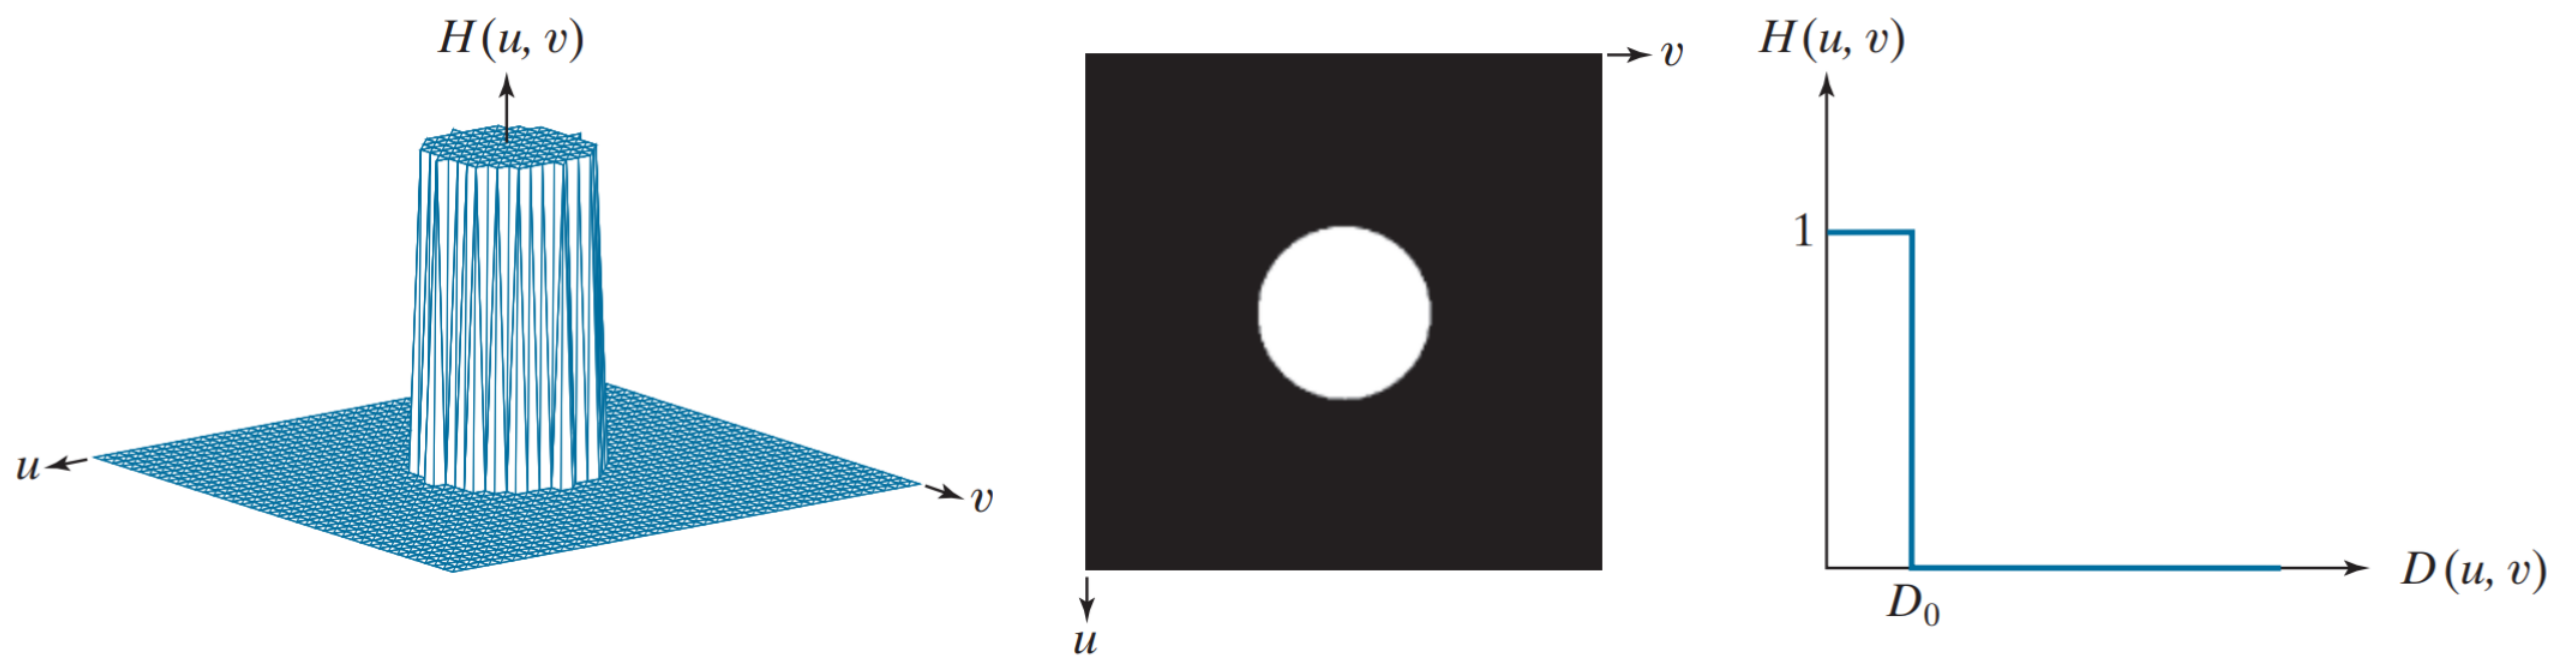
\includegraphics[width=\linewidth]{images/ideal_low_pass.png}
          \end{figure}
        \end{minipage}

        \begin{equation*}
          H(u, v) =
          \begin{cases}
            1 & \text{if } D(u, v) \leq D_0 \\
            0 & \text{otherwise}
          \end{cases}
        \end{equation*}

      \item \textbf{Butterworth Low-pass filter:} A smoother
        transition between the pass and stop bands than the ideal low-pass
        filter. With order $n$ and cutoff frequency $D_0$:

        \begin{minipage}{\linewidth}
          \begin{figure}[H]
            \centering
            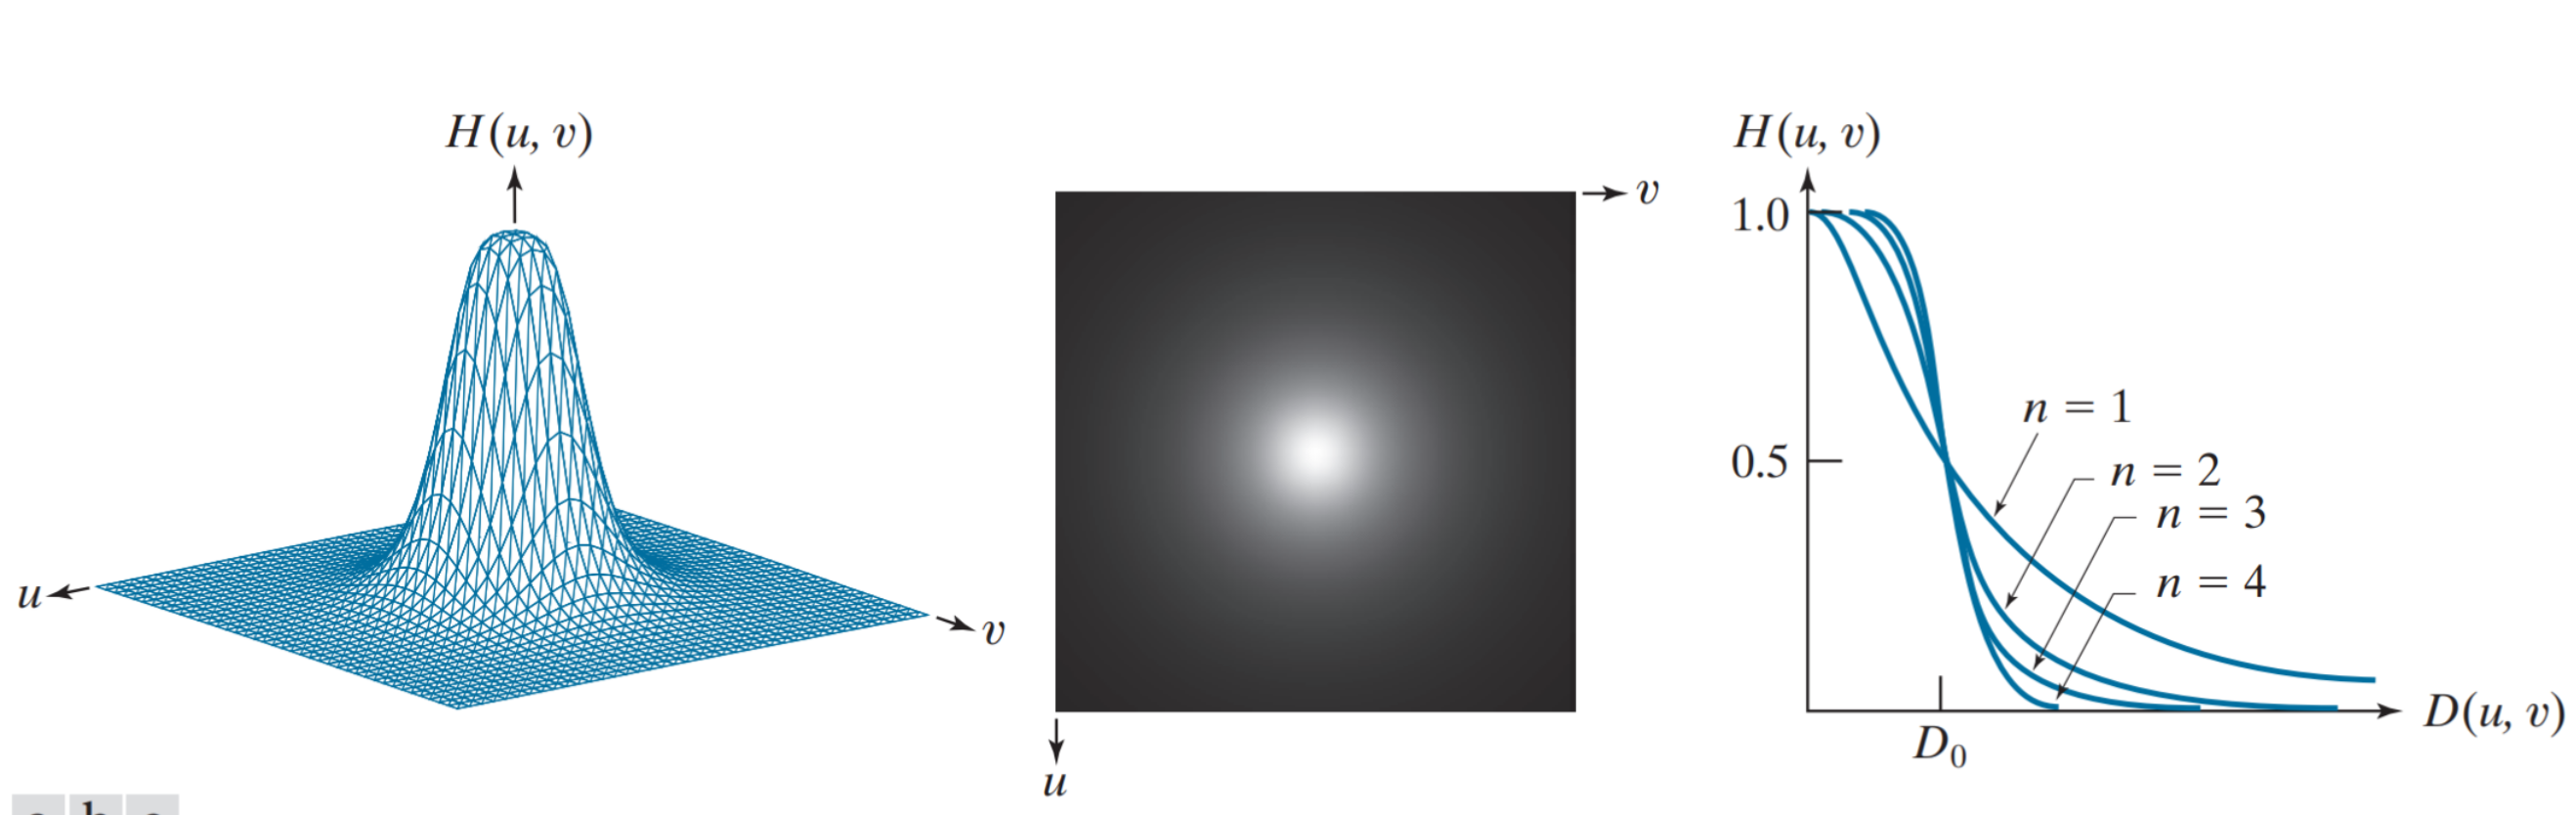
\includegraphics[width=\linewidth]{images/butterworth_low_pass.png}
          \end{figure}
        \end{minipage}

        \begin{equation*}
          H(u, v) = \frac{1}{1 + (D(u, v)/D_0)^{2n}}
        \end{equation*}

      \item \textbf{Gaussian Low-pass filter:} A Gaussian function
        that smoothly decays to zero as $D(u, v)$ increases. With cutoff
        frequency $D_0$:

        \begin{minipage}{\linewidth}
          \begin{figure}[H]
            \centering
            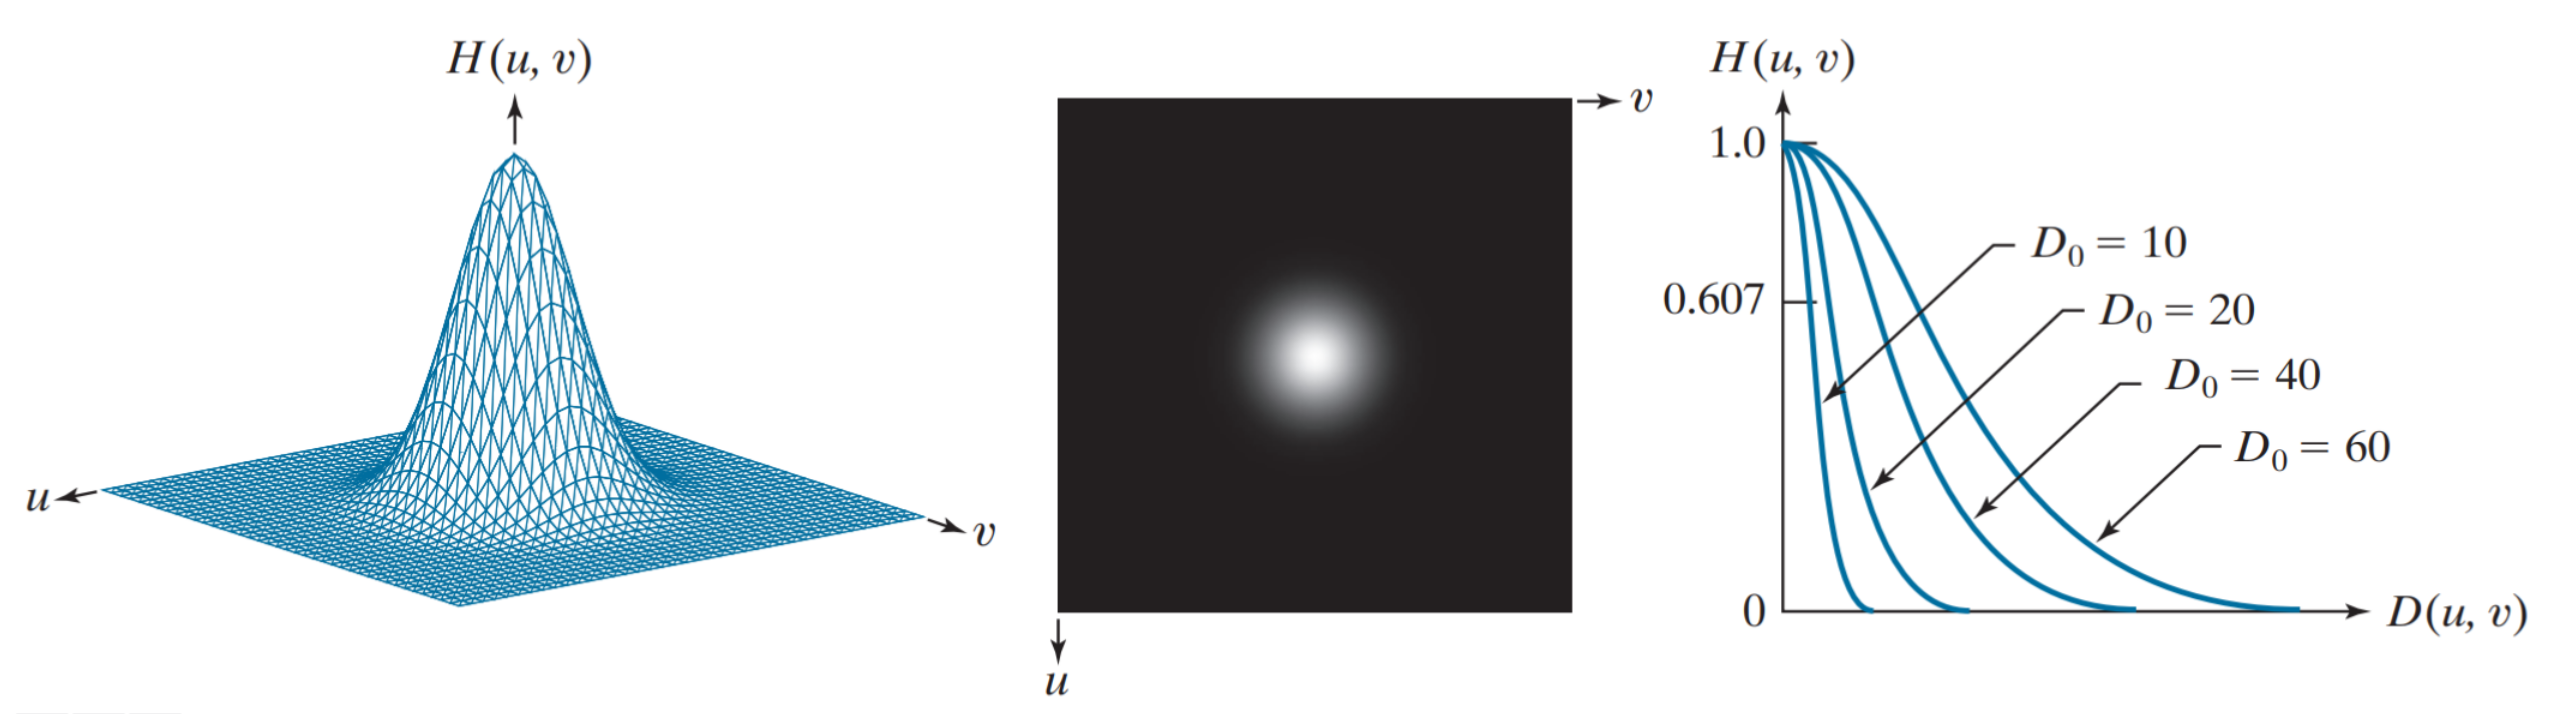
\includegraphics[width=\linewidth]{images/gaussian_low_pass.png}
          \end{figure}
        \end{minipage}

        \begin{equation*}
          H(u, v) = e^{-D(u, v)^2/2D_0^2}
        \end{equation*}

        \begin{itemize}
          \item Gaussian filters are often used to correct \textbf{broken
            characters} in low resolution text images.

            \begin{minipage}{\linewidth}
              \vspace{-0.5cm}
              \begin{figure}[H]
                \centering
                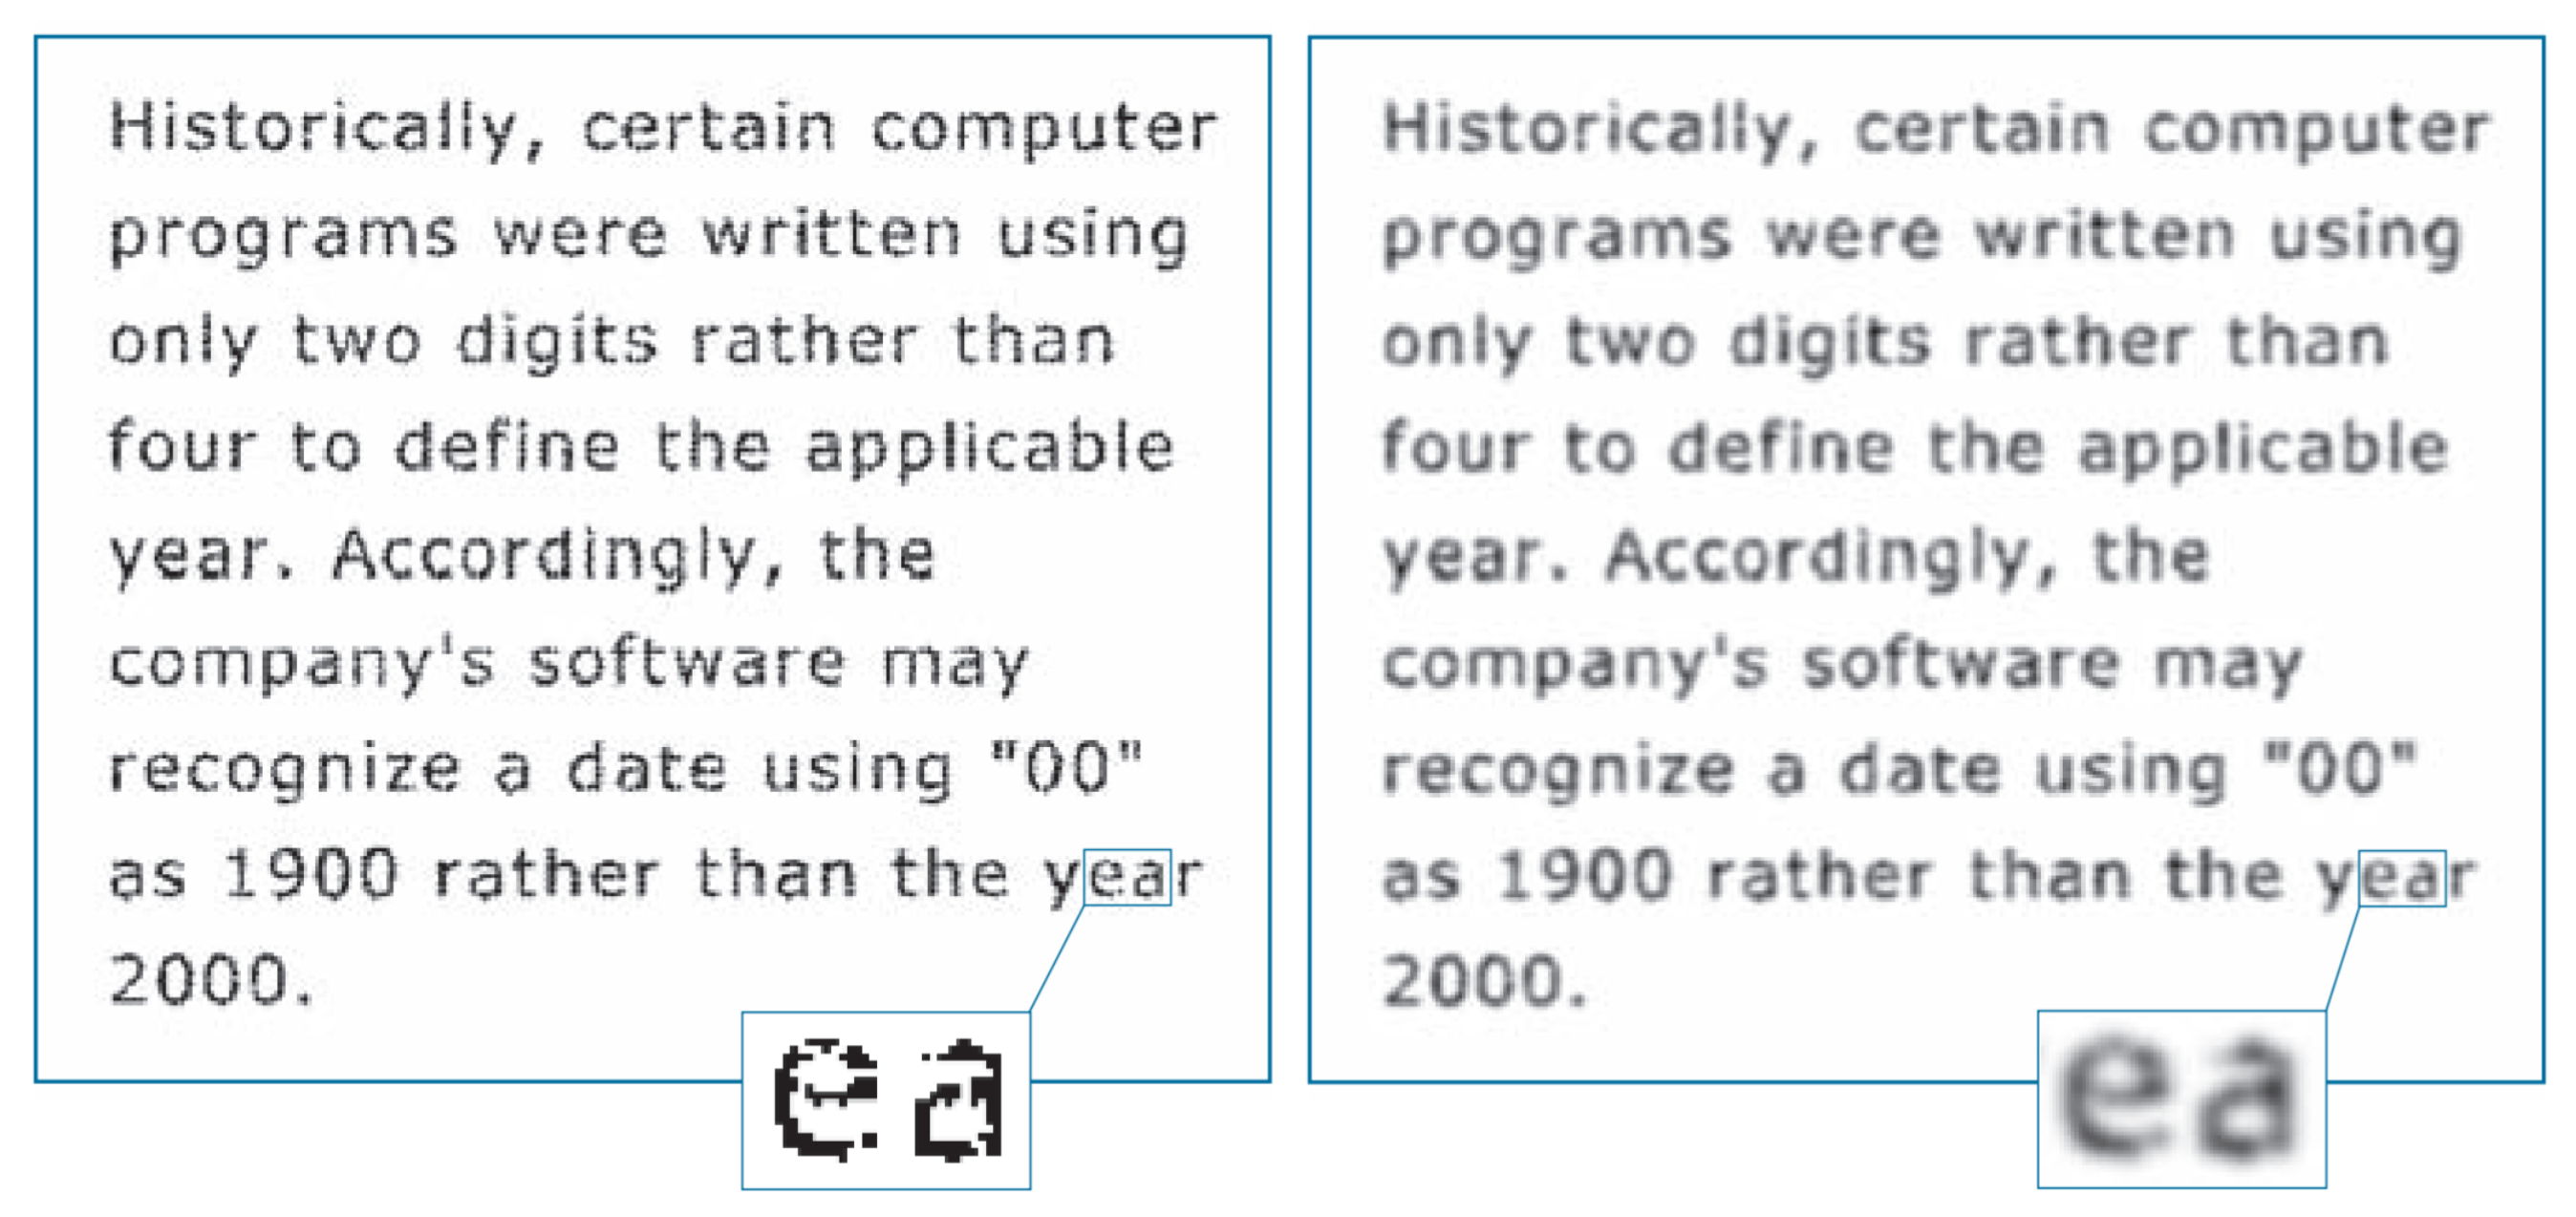
\includegraphics[width=\linewidth]{images/gaussian_text_correction.png}
                \caption{Gaussian filter can correct broken characters}
              \end{figure}
            \end{minipage}

          \item Gaussian filters can also \textbf{remove blemishes in
            photographs}

            \begin{minipage}{\linewidth}
              \vspace{-0.4cm}
              \begin{figure}[H]
                \centering
                \includegraphics[width=\linewidth]{images/gaussian_photo_correction.png}
                \caption{Gaussian filter can remove blemishes in photographs}
              \end{figure}
            \end{minipage}
        \end{itemize}
    \end{itemize}

  \item \textbf{Sharpening filters:} Edges and fine details are
    associated with high frequency components.

    \begin{itemize}
      \item \textbf{Ideal high-pass filter:} Cut off all low
        frequency components that are a specified distance $D_0$ from
        the origin of the transform.

        \begin{minipage}{\linewidth}
          \begin{figure}[H]
            \centering
            \includegraphics[width=\linewidth]{images/ideal_high_pass.png}
          \end{figure}
        \end{minipage}

        \begin{equation*}
          H_\text{hp}(u, v) = 1 - H_\text{lp}(u, v) =
          \begin{cases}
            0 & \text{if } D(u, v) \leq D_0 \\
            1 & \text{otherwise}
          \end{cases}
        \end{equation*}

      \item \textbf{Butterworth High-pass filter:} A smoother
        transition between the pass and stop bands than the ideal high-pass
        filter. With order $n$ and cutoff frequency $D_0$:

        \begin{minipage}{\linewidth}
          \begin{figure}[H]
            \centering
            \includegraphics[width=\linewidth]{images/butterworth_high_pass.png}
          \end{figure}
        \end{minipage}

        \begin{equation*}
          H_\text{hp}(u, v) = \frac{1}{1 + (D_0/D_(u, v))^{2n}}
        \end{equation*}

      \item \textbf{Gaussian High-pass filter:} A Gaussian function
        that smoothly increases to 1 as $D(u, v)$ increases. With cutoff
        frequency $D_0$:

        \begin{minipage}{\linewidth}
          \begin{figure}[H]
            \centering
            \includegraphics[width=\linewidth]{images/gaussian_high_pass.png}
          \end{figure}
        \end{minipage}

        \begin{equation*}
          H_\text{hp}(u, v) = 1 - e^{-D(u, v)^2/2D_0^2}
        \end{equation*}

    \end{itemize}
\end{itemize}

\subsection*{Fast Fourier Transform (FFT)}

\begin{itemize}
  \item DFT is computationally expensive, with a time complexity of
    $O((MN)^2)$, where M and N are the dimensions of the image
  \item \textbf{Fast Fourier Transform (FFT)} allows the Fourier
    transform to be carried out in a reasonable amount of time
  \item It reduces the amount of time required to complete a Fourier
    transform by a factor of \textbf{100 - 600 times}!
  \item FFT is the reason why Fourier based techniques have gained
    popularity in image processing
\end{itemize}

\subsection*{Spatial vs Frequency Domain}

\begin{itemize}
  \item Similar jobs can be done in both spatial and frequency domains
  \item Filtering in the spatial domain can be easier to understand
  \item Filtering in the frequency domain can be much faster –
    especially for large images
\end{itemize}
